\documentclass{standalone}
\usepackage{tikz}
\usetikzlibrary{patterns, positioning}
\usepackage[sfdefault]{ClearSans} %% option 'sfdefault' activates Clear Sans as the default text font
\usepackage[T1]{fontenc}

\begin{document}
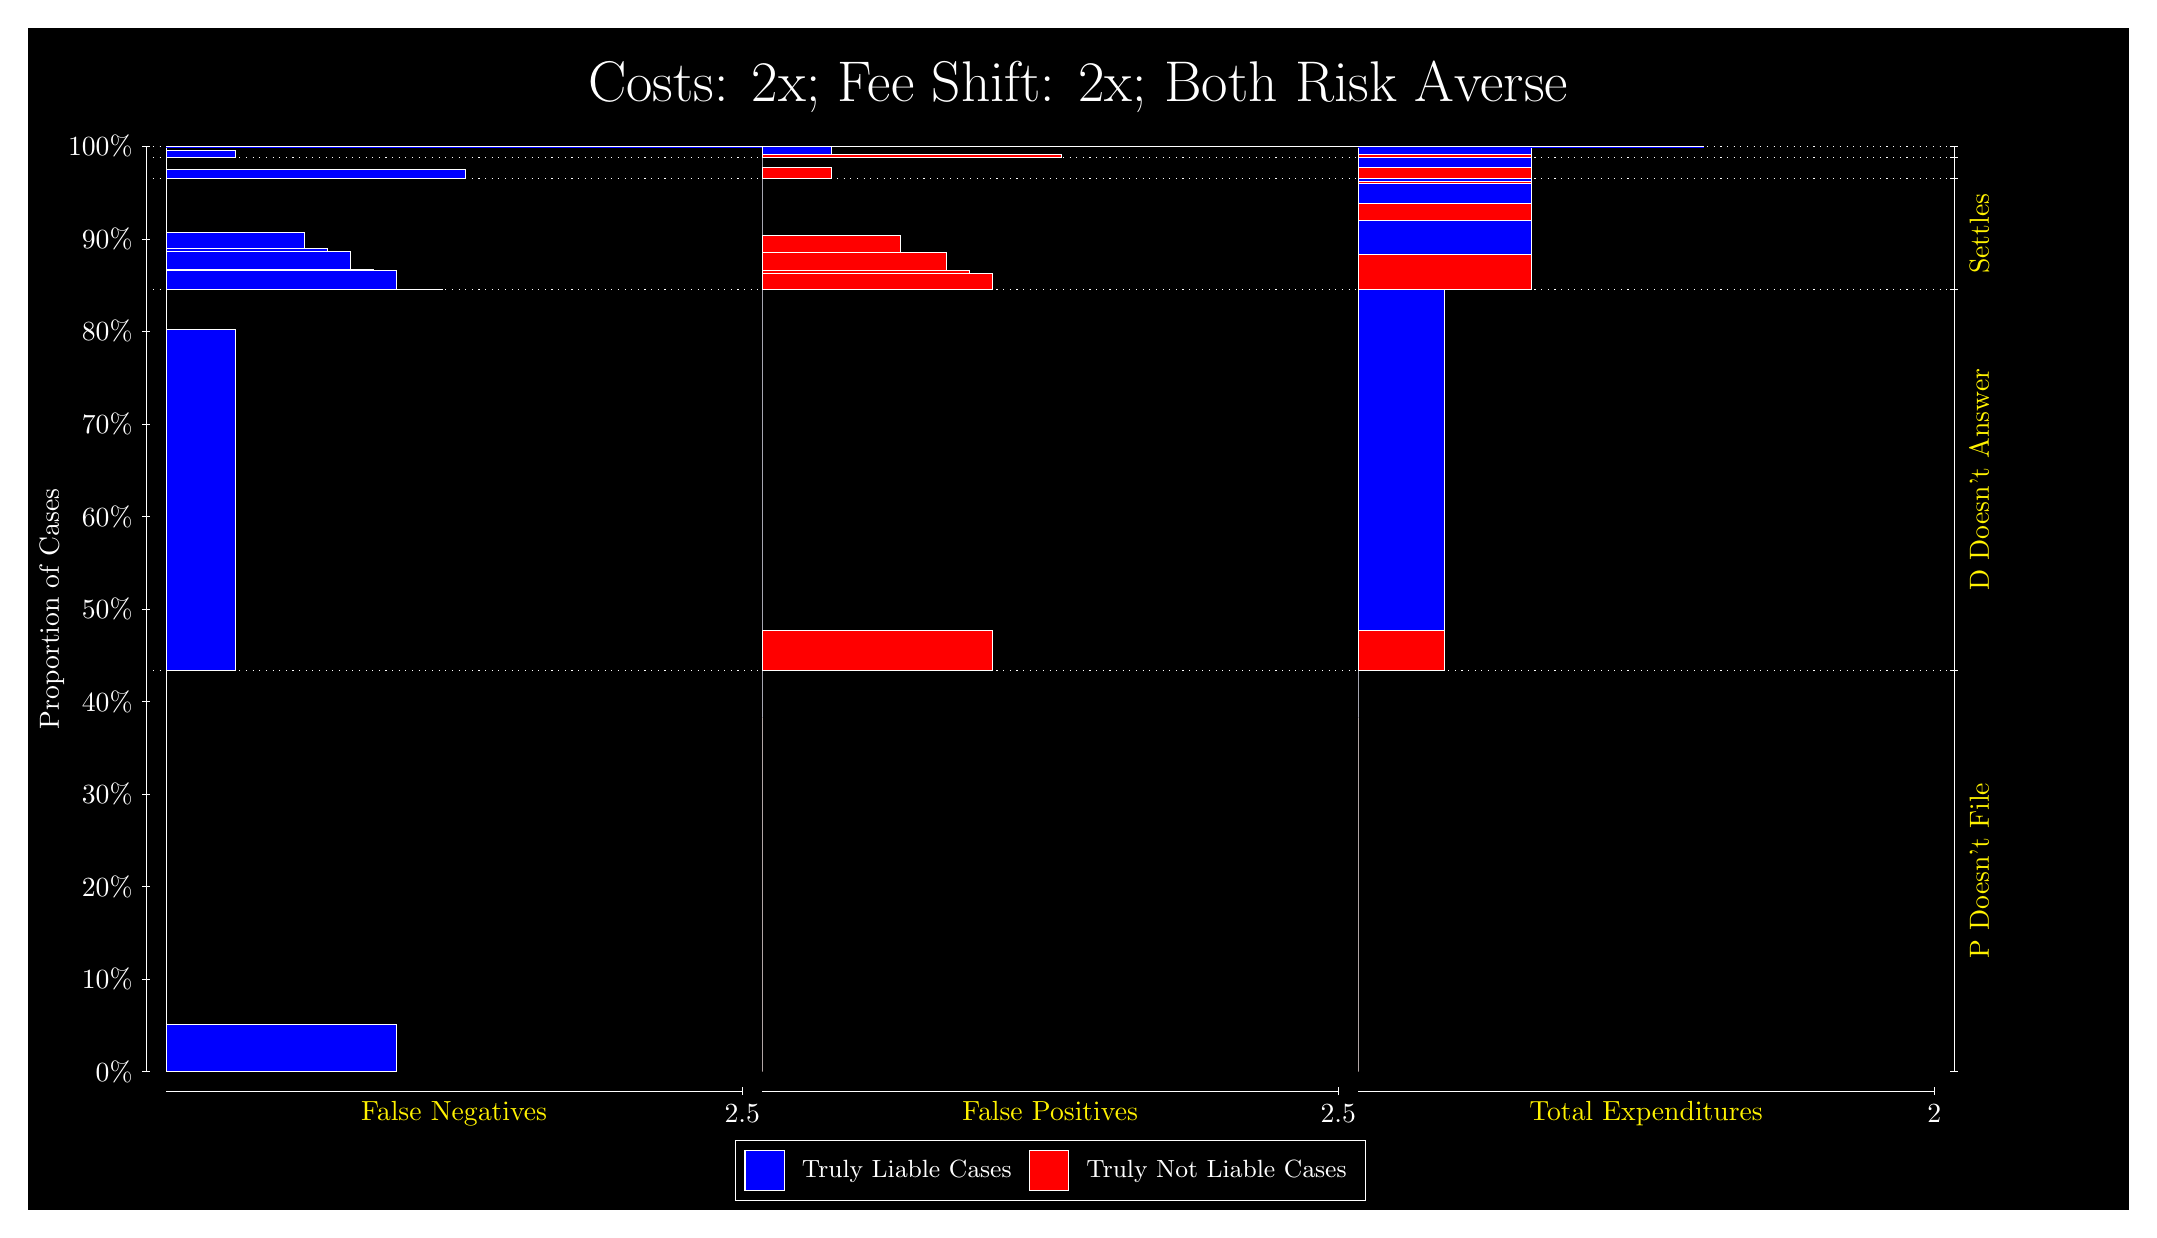
\begin{tikzpicture}
\draw[fill=black] (0,0) rectangle (26.667,15);
\draw[text=white] (0,13.5) rectangle (26.667,15) node[midway] {\huge Costs: 2x; Fee Shift: 2x; Both Risk Averse};
\draw[white, very thin] (1.5,1.75) -- (1.5,13.5);
\node[rotate=90, text=white, anchor=center] at (0.3, 7.625) {Proportion of Cases};
\draw[white, very thin] (1.45,1.75) -- (1.55,1.75);
\node[text=white, anchor=east] at (1.45, 1.75) {0\%};
\draw[white, very thin] (1.45,2.925) -- (1.55,2.925);
\node[text=white, anchor=east] at (1.45, 2.925) {10\%};
\draw[white, very thin] (1.45,4.1) -- (1.55,4.1);
\node[text=white, anchor=east] at (1.45, 4.1) {20\%};
\draw[white, very thin] (1.45,5.275) -- (1.55,5.275);
\node[text=white, anchor=east] at (1.45, 5.275) {30\%};
\draw[white, very thin] (1.45,6.45) -- (1.55,6.45);
\node[text=white, anchor=east] at (1.45, 6.45) {40\%};
\draw[white, very thin] (1.45,7.625) -- (1.55,7.625);
\node[text=white, anchor=east] at (1.45, 7.625) {50\%};
\draw[white, very thin] (1.45,8.8) -- (1.55,8.8);
\node[text=white, anchor=east] at (1.45, 8.8) {60\%};
\draw[white, very thin] (1.45,9.975) -- (1.55,9.975);
\node[text=white, anchor=east] at (1.45, 9.975) {70\%};
\draw[white, very thin] (1.45,11.15) -- (1.55,11.15);
\node[text=white, anchor=east] at (1.45, 11.15) {80\%};
\draw[white, very thin] (1.45,12.325) -- (1.55,12.325);
\node[text=white, anchor=east] at (1.45, 12.325) {90\%};
\draw[white, very thin] (1.45,13.5) -- (1.55,13.5);
\node[text=white, anchor=east] at (1.45, 13.5) {100\%};

\draw[white, very thin] (24.457,1.75) -- (24.457,13.5);
\draw[white, very thin] (24.407,1.75) -- (24.507,1.75);
\node[anchor=west] at (24.407, 1.75) {};
\draw[white, very thin] (24.407,6.8481) -- (24.507,6.8481);
\node[anchor=west] at (24.407, 6.8481) {};
\draw[white, very thin] (24.407,11.684) -- (24.507,11.684);
\node[anchor=west] at (24.407, 11.684) {};
\draw[white, very thin] (24.407,13.096) -- (24.507,13.096);
\node[anchor=west] at (24.407, 13.096) {};
\draw[white, very thin] (24.407,13.357) -- (24.507,13.357);
\node[anchor=west] at (24.407, 13.357) {};
\draw[white, very thin] (24.407,13.495) -- (24.507,13.495);
\node[anchor=west] at (24.407, 13.495) {};
\draw[white, very thin] (24.407,13.497) -- (24.507,13.497);
\node[anchor=west] at (24.407, 13.497) {};
\draw[white, very thin] (24.407,13.5) -- (24.507,13.5);
\node[anchor=west] at (24.407, 13.5) {};

\draw[white, very thin, fill=blue] (1.75,1.75) rectangle (4.6775,2.3549);
\draw[white, very thin, fill=red] (1.75,2.3549) rectangle (1.75,6.8481);
\draw[white, very thin, fill=blue] (1.75,6.8481) rectangle (2.6283,11.178);
\draw[white, very thin, fill=red] (1.75,11.178) rectangle (1.75,11.684);
\draw[white, very thin, fill=blue] (1.75,11.684) rectangle (5.2631,11.685);
\draw[white, very thin, fill=blue] (1.75,11.685) rectangle (4.9703,11.685);
\draw[white, very thin, fill=blue] (1.75,11.685) rectangle (4.6775,11.932);
\draw[white, very thin, fill=blue] (1.75,11.932) rectangle (4.3848,11.933);
\draw[white, very thin, fill=blue] (1.75,11.933) rectangle (4.092,12.171);
\draw[white, very thin, fill=blue] (1.75,12.171) rectangle (3.7993,12.205);
\draw[white, very thin, fill=blue] (1.75,12.205) rectangle (3.5065,12.41);
\draw[white, very thin, fill=red] (1.75,12.41) rectangle (1.75,13.096);
\draw[white, very thin, fill=blue] (1.75,13.096) rectangle (5.5558,13.213);
\draw[white, very thin, fill=red] (1.75,13.213) rectangle (1.75,13.357);
\draw[white, very thin, fill=blue] (1.75,13.357) rectangle (2.6283,13.45);
\draw[white, very thin, fill=red] (1.75,13.45) rectangle (1.75,13.495);
\draw[white, very thin, fill=blue] (1.75,13.495) rectangle (9.9471,13.496);
\draw[white, very thin, fill=red] (1.75,13.496) rectangle (1.75,13.497);
\draw[white, very thin, fill=red] (1.75,13.497) rectangle (1.75,13.498);
\draw[white, very thin, fill=blue] (1.75,13.498) rectangle (1.75,13.5);
\draw[white, very thin, fill=red] (9.3189,1.75) rectangle (9.3189,6.2432);
\draw[white, very thin, fill=blue] (9.3189,6.2432) rectangle (9.3189,6.8481);
\draw[white, very thin, fill=red] (9.3189,6.8481) rectangle (12.246,7.3536);
\draw[white, very thin, fill=blue] (9.3189,7.3536) rectangle (9.3189,11.684);
\draw[white, very thin, fill=red] (9.3189,11.684) rectangle (12.246,11.889);
\draw[white, very thin, fill=red] (9.3189,11.889) rectangle (11.954,11.92);
\draw[white, very thin, fill=red] (9.3189,11.92) rectangle (11.661,12.155);
\draw[white, very thin, fill=red] (9.3189,12.155) rectangle (11.368,12.156);
\draw[white, very thin, fill=red] (9.3189,12.156) rectangle (11.075,12.368);
\draw[white, very thin, fill=red] (9.3189,12.368) rectangle (10.783,12.368);
\draw[white, very thin, fill=red] (9.3189,12.368) rectangle (10.49,12.369);
\draw[white, very thin, fill=blue] (9.3189,12.369) rectangle (9.3189,13.096);
\draw[white, very thin, fill=red] (9.3189,13.096) rectangle (10.197,13.239);
\draw[white, very thin, fill=blue] (9.3189,13.239) rectangle (9.3189,13.357);
\draw[white, very thin, fill=red] (9.3189,13.357) rectangle (13.125,13.402);
\draw[white, very thin, fill=blue] (9.3189,13.402) rectangle (10.197,13.495);
\draw[white, very thin, fill=red] (9.3189,13.495) rectangle (9.3189,13.496);
\draw[white, very thin, fill=blue] (9.3189,13.496) rectangle (9.3189,13.497);
\draw[white, very thin, fill=red] (9.3189,13.497) rectangle (17.516,13.498);
\draw[white, very thin, fill=blue] (9.3189,13.498) rectangle (14.588,13.5);
\draw[white, very thin, fill=red] (16.888,1.75) rectangle (16.888,6.2432);
\draw[white, very thin, fill=blue] (16.888,6.2432) rectangle (16.888,6.8481);
\draw[white, very thin, fill=red] (16.888,6.8481) rectangle (17.986,7.3536);
\draw[white, very thin, fill=blue] (16.888,7.3536) rectangle (17.986,11.684);
\draw[white, very thin, fill=red] (16.888,11.684) rectangle (19.083,12.124);
\draw[white, very thin, fill=blue] (16.888,12.124) rectangle (19.083,12.566);
\draw[white, very thin, fill=red] (16.888,12.566) rectangle (19.083,12.78);
\draw[white, very thin, fill=blue] (16.888,12.78) rectangle (19.083,13.03);
\draw[white, very thin, fill=red] (16.888,13.03) rectangle (19.083,13.062);
\draw[white, very thin, fill=blue] (16.888,13.062) rectangle (19.083,13.096);
\draw[white, very thin, fill=red] (16.888,13.096) rectangle (19.083,13.239);
\draw[white, very thin, fill=blue] (16.888,13.239) rectangle (19.083,13.357);
\draw[white, very thin, fill=red] (16.888,13.357) rectangle (19.083,13.402);
\draw[white, very thin, fill=blue] (16.888,13.402) rectangle (19.083,13.495);
\draw[white, very thin, fill=red] (16.888,13.495) rectangle (21.279,13.496);
\draw[white, very thin, fill=blue] (16.888,13.496) rectangle (21.279,13.497);
\draw[white, very thin, fill=red] (16.888,13.497) rectangle (21.279,13.498);
\draw[white, very thin, fill=blue] (16.888,13.498) rectangle (21.279,13.5);
\draw[white, dotted] (1.5,6.8481) -- (24.457,6.8481);
\draw[white, dotted] (1.5,11.684) -- (24.457,11.684);
\draw[white, dotted] (1.5,13.096) -- (24.457,13.096);
\draw[white, dotted] (1.5,13.357) -- (24.457,13.357);
\draw[white, dotted] (1.5,13.495) -- (24.457,13.495);
\draw[white, dotted] (1.5,13.497) -- (24.457,13.497);
\draw[white, very thin] (1.75,1.5) -- (9.0689,1.5);
\node[text=yellow, anchor=north] at (5.4094, 1.5) {False Negatives};
\draw[white, very thin] (9.0689,1.45) -- (9.0689,1.55);
\node[text=white, anchor=north] at (9.0689, 1.45) {2.5};

\draw[white, very thin] (9.3189,1.5) -- (16.638,1.5);
\node[text=yellow, anchor=north] at (12.978, 1.5) {False Positives};
\draw[white, very thin] (16.638,1.45) -- (16.638,1.55);
\node[text=white, anchor=north] at (16.638, 1.45) {2.5};

\draw[white, very thin] (16.888,1.5) -- (24.207,1.5);
\node[text=yellow, anchor=north] at (20.547, 1.5) {Total Expenditures};
\draw[white, very thin] (24.207,1.45) -- (24.207,1.55);
\node[text=white, anchor=north] at (24.207, 1.45) {2};

\node[text=yellow, centered, rotate=90] at (24.777, 4.2991) {P Doesn't File};
\node[text=yellow, centered, rotate=90] at (24.777, 9.2659) {D Doesn't Answer};
\node[text=yellow, centered, rotate=90] at (24.777, 12.39) {Settles};





\draw (12.978300999999998,1.5) node[draw=none] (baseCoordinate) {};
\begin{scope}[align=center]
        \matrix[scale=0.5, draw=white, below=0.5cm of baseCoordinate, nodes={draw}, column sep=0.1cm]{
            \node[rectangle, draw, minimum width=0.5cm, minimum height=0.5cm, fill=blue] {}; &
            \node[draw=none, font=\small, text=white] (B) {Truly Liable Cases}; &
            \node[rectangle, draw, minimum width=0.5cm, minimum height=0.5cm, fill=red] {}; &
            \node[draw=none, font=\small, text=white] (B) {Truly Not Liable Cases}; \\
            };
\end{scope}

\end{tikzpicture}
\end{document}